\chapter{The Probably Approximately Correct Learning Model}
    \section{A Rectangular Learning Game}
    \begin{figure}[h]
        \begin{center}
            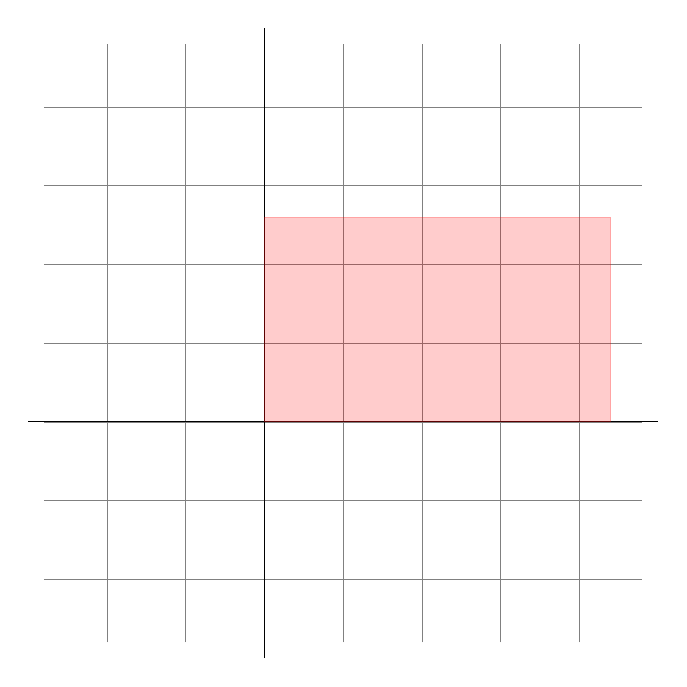
\begin{tikzpicture}[scale=2]
                \draw[step=.5cm,gray,very thin] (-1.4,-1.4) grid (2.4,2.4);
                \draw (-1.5,0) -- (2.5,0);
                \draw (0,-1.5) -- (0,2.5);
                \filldraw[red, opacity=.2] rectangle (2.2, 1.3) (.7,2.2);
                % dot
                % \node[fill=black,draw=black,circle,circle radius=1] (A) at (1.7,2) {};
            \end{tikzpicture}
        \end{center}
        \caption{A rectangular learning game}
    \end{figure}
